\documentclass{article}

\usepackage{array}
\usepackage{graphicx}

\begin{document}

\title{Capacitors, Resistors and Current}
\author{GSI: Caleb Eades}
\date{10/18}
\maketitle

\section{Capacitors}

Note: the solutions to these problems are 1.1 and 1.2 of capacitorssol.pdf.

\subsection{Cylindrical Capacitor}

Calculate the capacitance of a pair of cylinders of radii $a$ and $b$ and length $l$. What is the energy stored in the capacitor? (Calculate this using both $U=CV^2/2$ and integrating the energy density $\epsilon=\epsilon_0\vec{E}^2/2$ over the volume between the plates.)

\subsection{Different Dielectrics}

A parallel-plate capacitor is filled with two different dielectrics as shown. The distance between the plates is $d$, the area of each plate is $A$ and the height of each dielectric is $b$.
\begin{enumerate}
	\item Assume that the charge on the plates is $\pm Q$ and find $\vec{E}$ in each of the four regions.
	\item Find the potential difference $V$ between the plates by integrating $\vec{E}$. 
	\item Compute the capacitance.
\end{enumerate}
\begin{figure}
	\begin{center}
	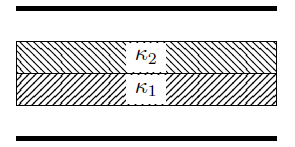
\includegraphics[width=0.5\textwidth]{MixedDielectrics.png}
	\end{center}
\end{figure}

(\textit{Source: modified from Vetri and Dan})

\end{document}
